\subsection{Gradient Descent}
\label{sec:gradient-descent}
Gradient descent is a first order optimization method, which means that it uses the first derivative of the function to find the minimum. The algorithm works by taking steps in the opposite direction of the gradient of the function, which is the direction of the steepest descent. The step size is controlled by the learning rate, which is a hyperparameter.

If the learning rate is too big then the gradient descent can overshoot the minimum and only then adjust to convergence. If the learning rate is too small then the gradient will take more iterations to converge but for convex functions the gradient descent will always converge at some point given enough steps \ref{fig:gd-hypersphere}.

\begin{figure}[H]
    \begin{subfigure}{0.5\linewidth}
        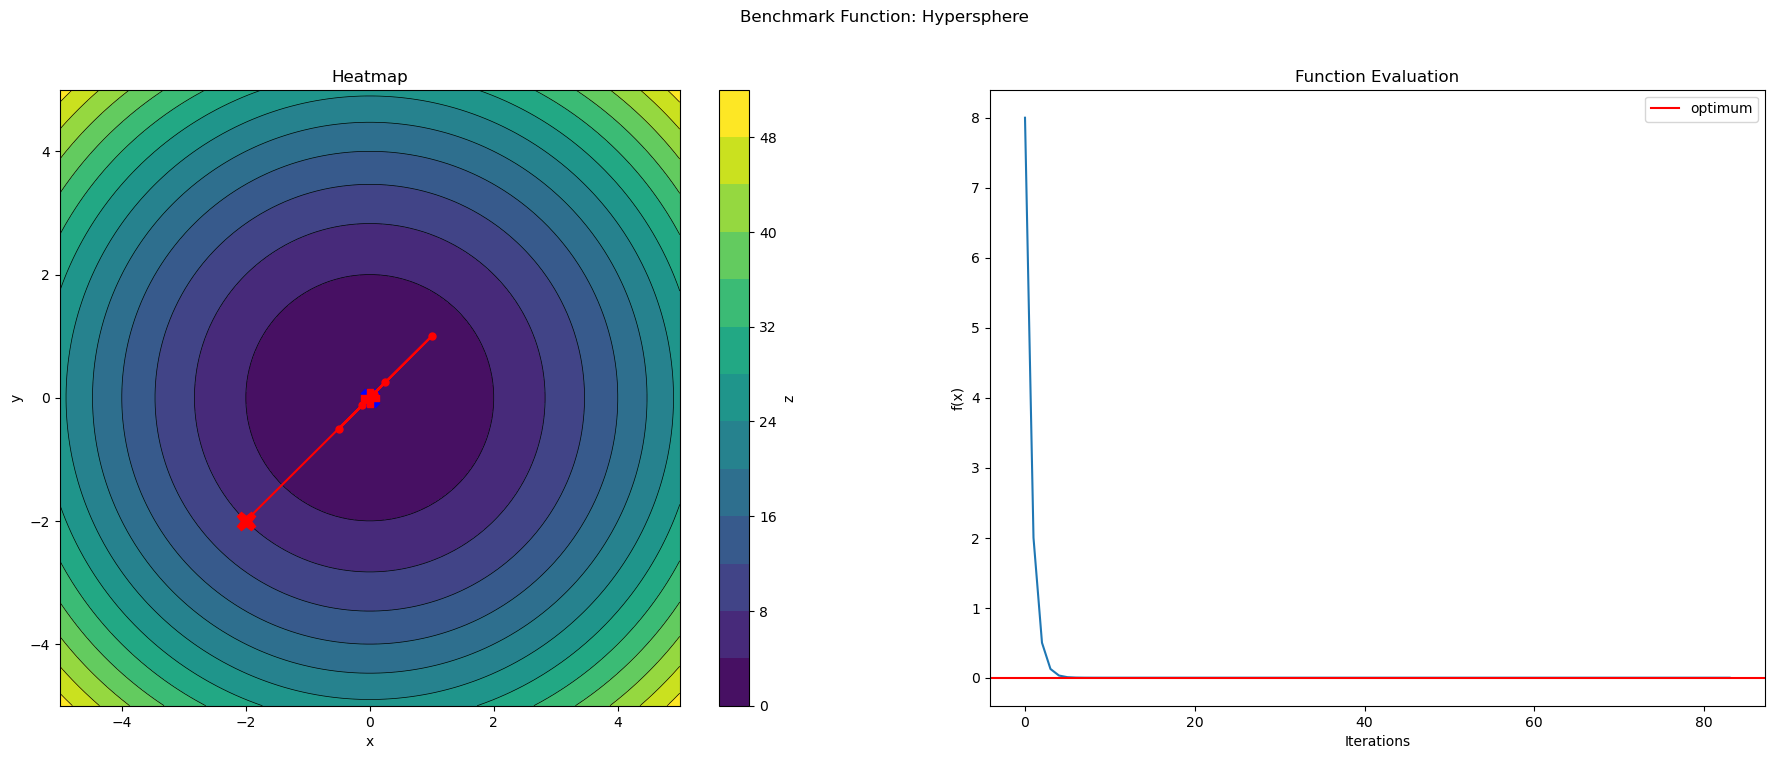
\includegraphics[width=\linewidth]{lab3/imgs/gd_sphere_75.png}
        \caption{Gradient descent with learning rate 0.75}
    \end{subfigure}
    \begin{subfigure}{0.5\linewidth}
        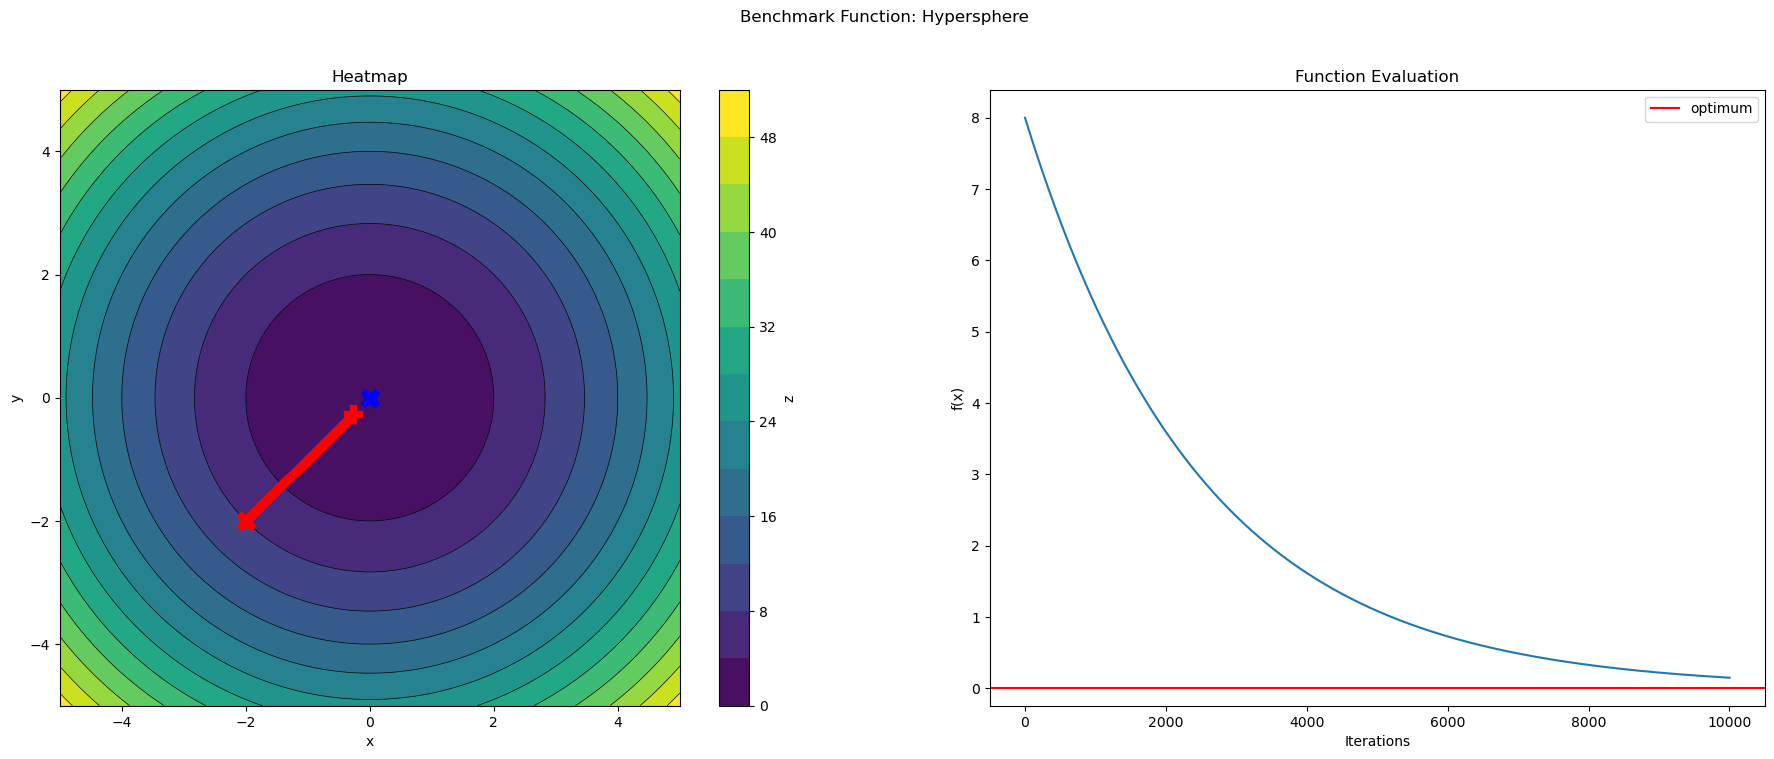
\includegraphics[width=\linewidth]{lab3/imgs/gd_sphere_04.png}
        \caption{Gradient descent with learning rate 0.4}
    \end{subfigure}
    \caption{Gradient descent on a 2D hypersphere}
    \label{fig:gd-hypersphere}
\end{figure}

For multimodal functions (many local minima), the gradient descent is only guaranteed to converge to the nearest local minimum, thus the starting point is very important.
\begin{figure}[H]
    \begin{subfigure}{0.5\linewidth}
        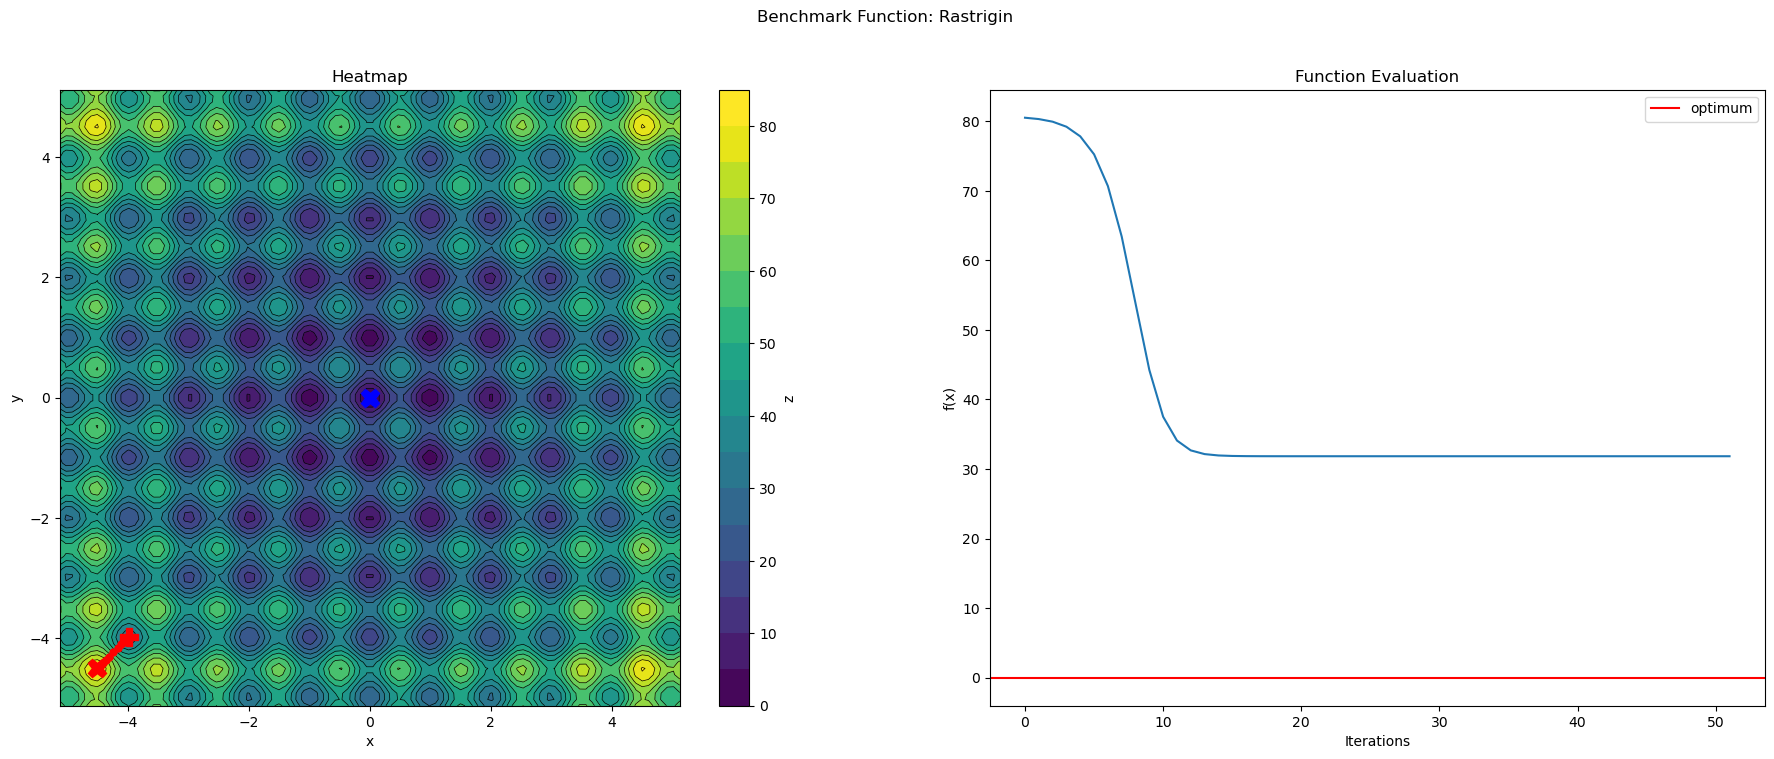
\includegraphics[width=\linewidth]{lab3/imgs/gd_rastr_local.png}
        \caption{Starting point[-4.5,-4.5]}
    \end{subfigure}
    \begin{subfigure}{0.5\linewidth}
        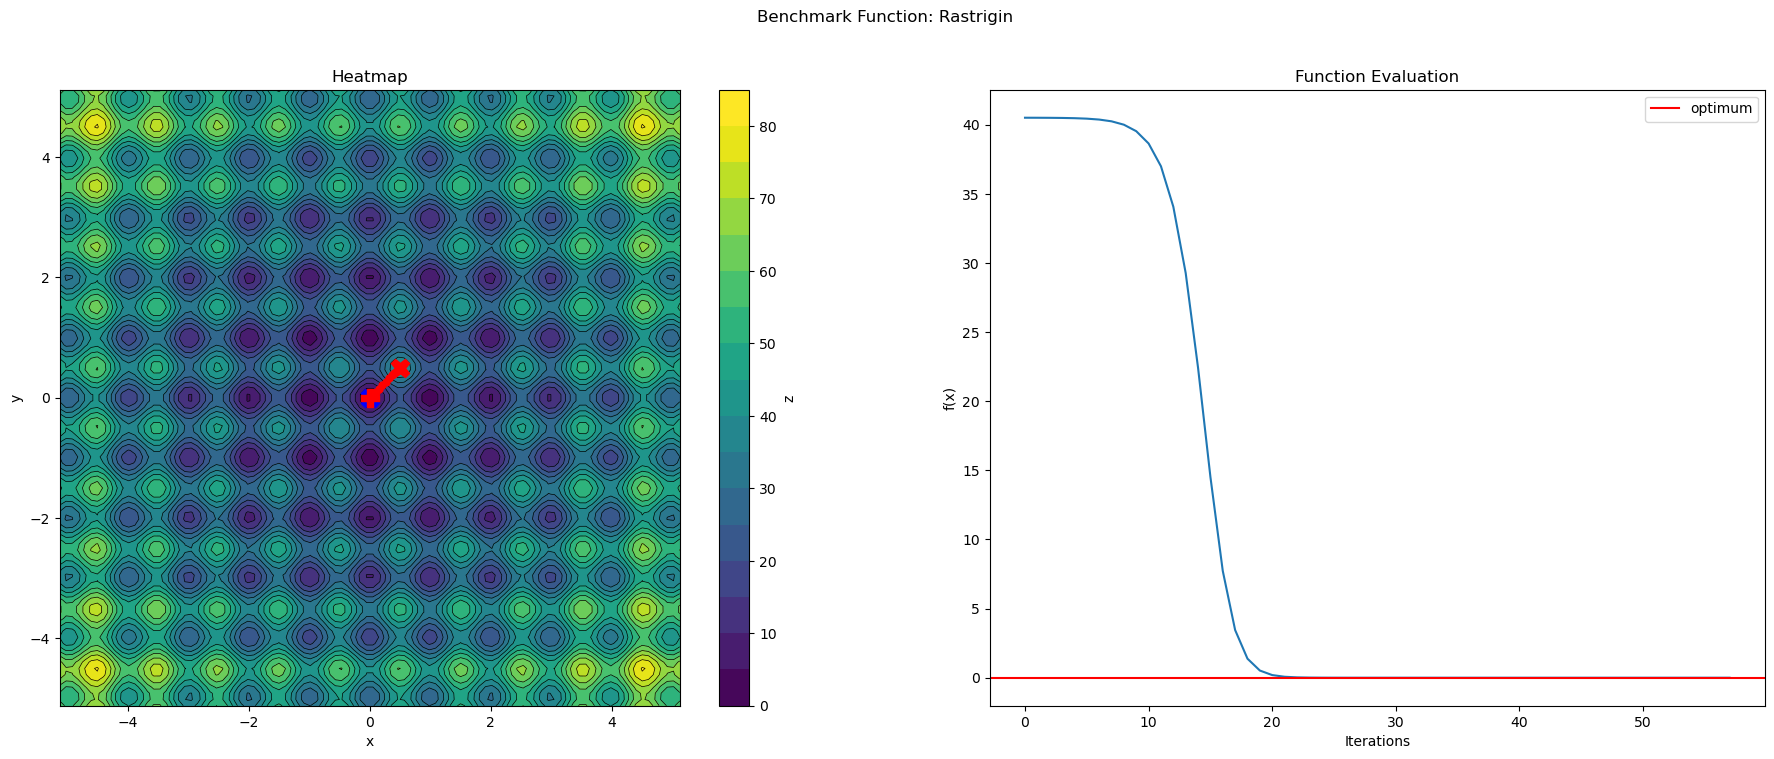
\includegraphics[width=\linewidth]{lab3/imgs/gd_rastr_global.png}
        \caption{Starting point [0.5,0.5]}
    \end{subfigure}
    \caption{Gradient descent on the Rastrigin function}
    \label{fig:gd-rastr}
\end{figure}

It the learning rate is large, gradient descent can also lead to numerical instability and overflow \ref{fig:ros-div}.
\begin{figure}[H]
    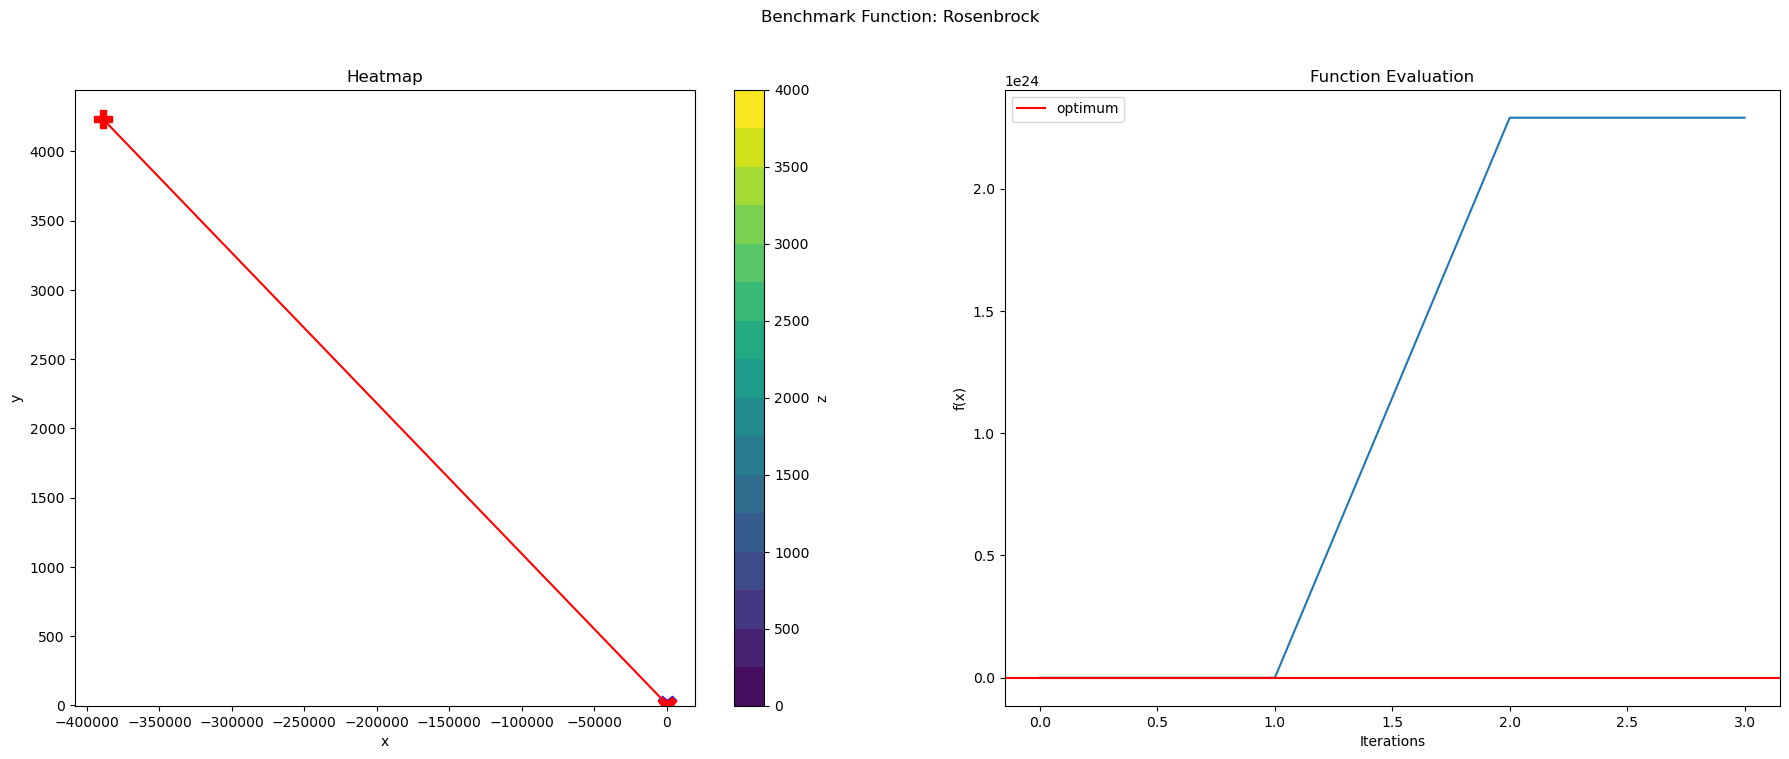
\includegraphics[width=\linewidth]{lab3/imgs/gd_rosenbrock_divergence.png}
    \caption{Gradient descent with learning rate 0.01 on the Rosenbrock function. The algorithm diverges.}
    \label{fig:ros-div}
\end{figure}



\subsection{Newton's Method}
\label{sec:newtons-method}
Newton's method is a second order optimization method, which means that it uses the second derivative of the function to find the minimum. Thus it's more informative than the gradient descent (it doesn't just use the slope of the function, but also the curvature). It can converge faster than gradient descent but it's computationally expensive since it needs to compute the inverse of the Hessian matrix.

Moreover, it has the advantage of having one less parameter to tune (the learning rate) since the algorithm uses instead information about the second derivate of the function to compute the step size.
Even if convergence is on average faster, the same convergence guarantees as the gradient descent apply.


\subsection{BFGS}
\label{sec:bfgs}
BFGS is a quasi-Newton method, which means that it's a second order optimization method that doesn't need to compute the Hessian matrix. It's a good compromise between the gradient descent and Newton's method, since it's faster than the gradient descent but doesn't have the same overhead of computing the Hessian matrix as Newton's methods.

Below \ref{fig:ros-comparison} we report an comparison between the three methods on the Rosenbrock function starting from point [2.0,2.0] and compare the number of iterations needed. It's interesting to notice that the BFGS terminates before reaching the global minimum and even changing the tolerance doesn't help in this case. Nevertheless, we obtain the expected result where the Newton's method converges in the fewest iterations, followed by the BFGS and then gradient descent.
\begin{figure}
    \begin{subfigure}{0.5\linewidth}
        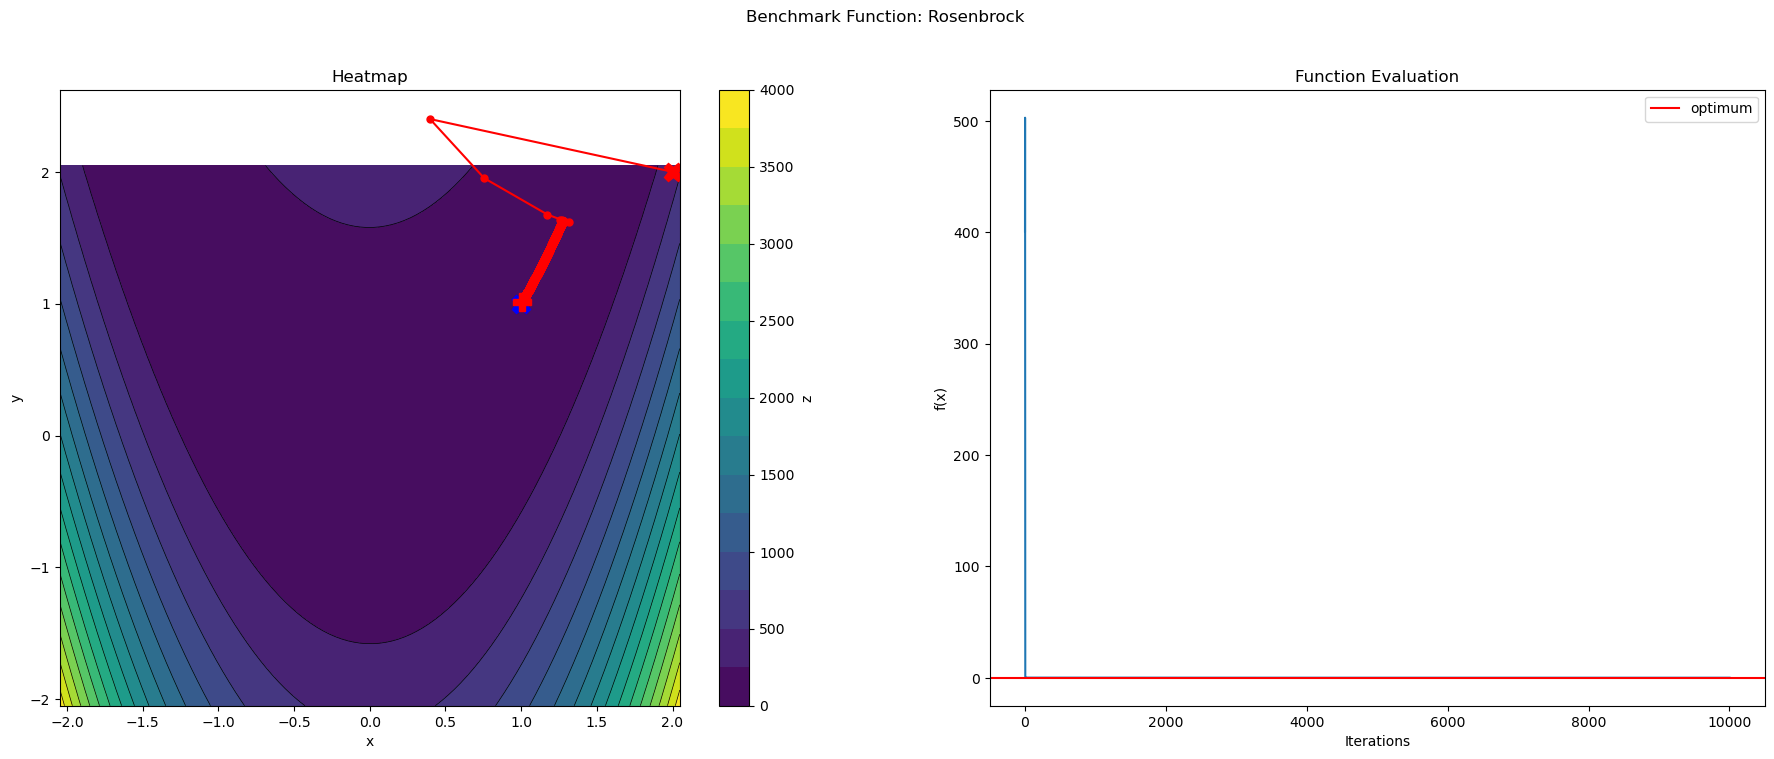
\includegraphics[width=\linewidth]{lab3/imgs/gd_rosenbrock.png}
        \caption{Gradient descent (10000 iterations)}
    \end{subfigure}
    \begin{subfigure}{0.5\linewidth}
        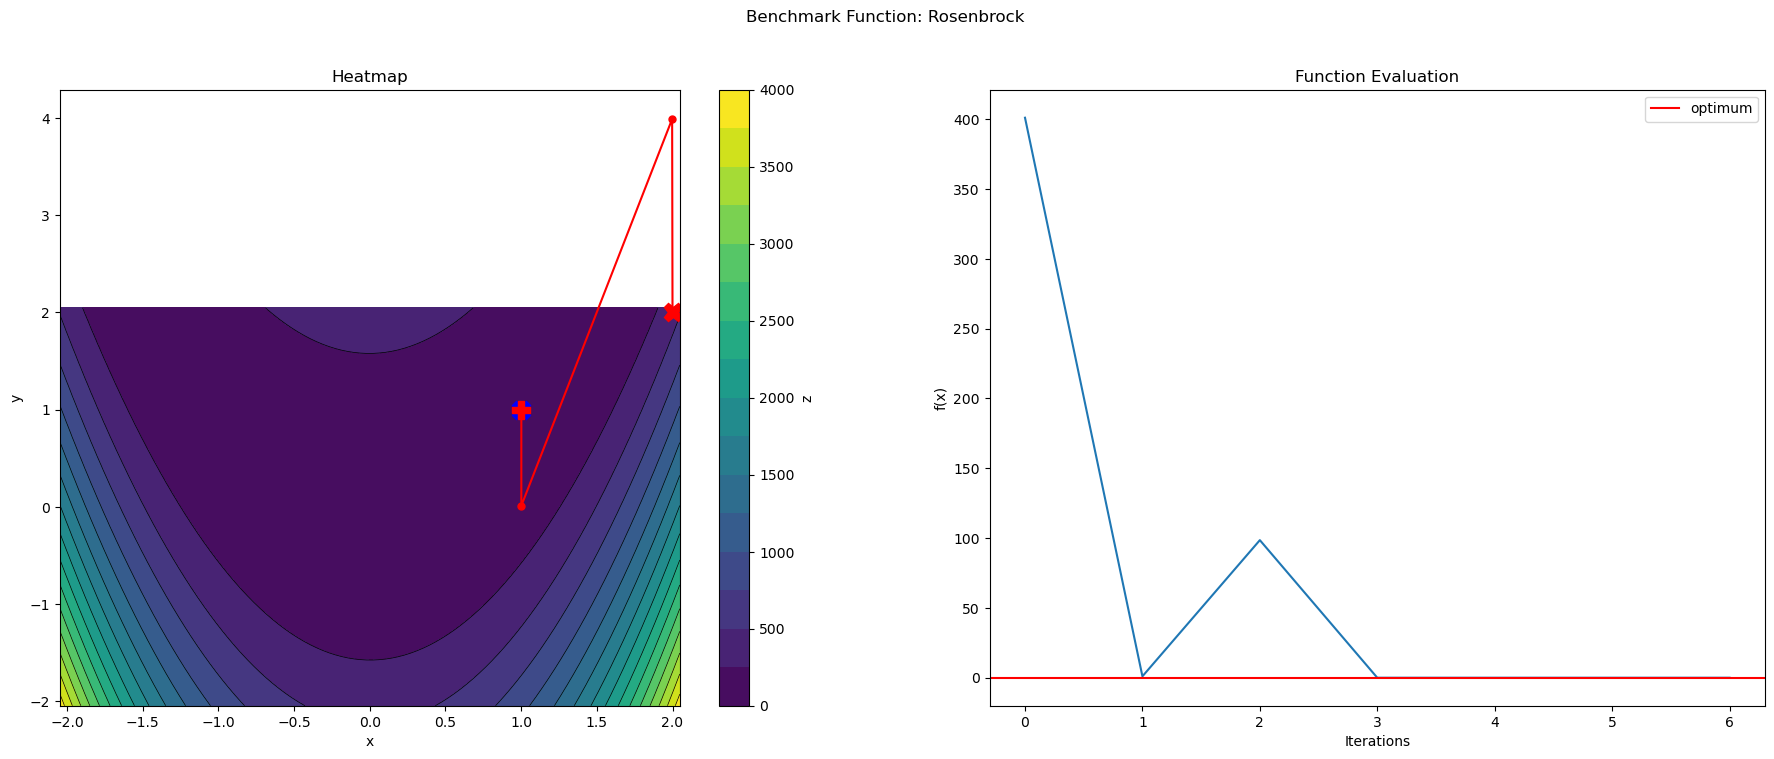
\includegraphics[width=\linewidth]{lab3/imgs/nm_rosenbrock.png}
        \caption{Newton's method (7 iterations)}
    \end{subfigure} \\
    \begin{subfigure}{\linewidth}
        \centering
        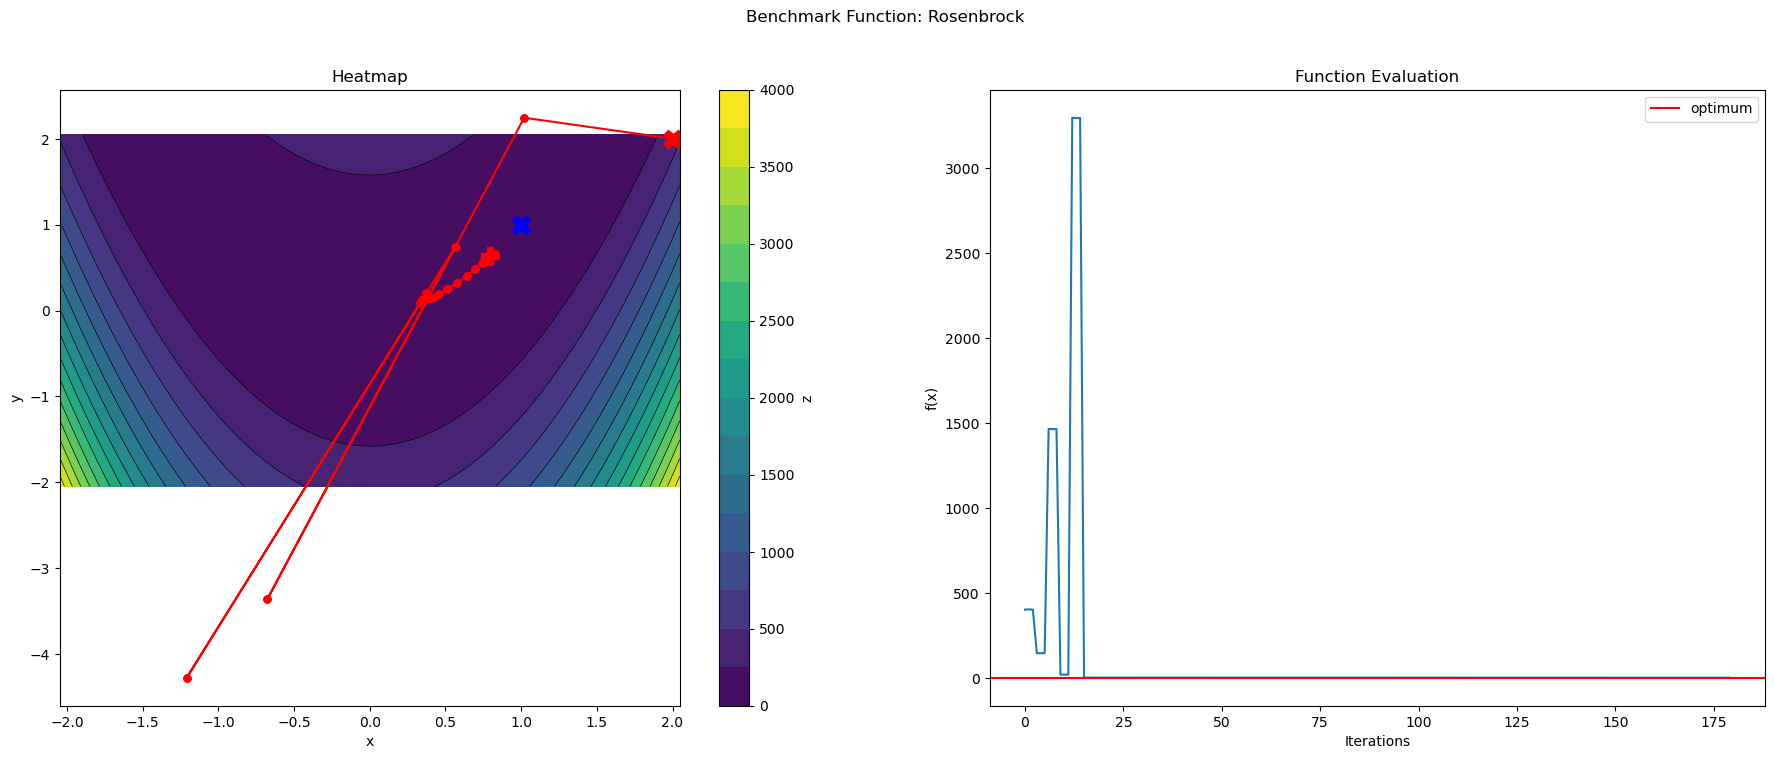
\includegraphics[width=0.5\linewidth]{lab3/imgs/bfgs_rosenbrock.png}
        \caption{BFGS (92 iterations)}
    \end{subfigure}
    \caption{Comparison between Gradient Descent, Newton's Method and BFGS on the Rosenbrock function}
    \label{fig:ros-comparison}
\end{figure}